\subsection{Free energy profile of basic patch}
In the context of the investigation of FAK falling the free energy profile of the basic patch in F2 was investigated. Because this might be of interest for other applications as well, a short report on the obtained results is given at this point. The used setup is setup 2 described in \autoref{setup:setup2}.\\
The average profile of the five copies together with the standard deviation for the forcefields C36, Martini and Martini with PW can be found in \autoref{umbrella:profiles}. Here the range between $z = 6\,\si{\nano\metre}$ and $z = 7\,\si{\nano\metre}$ was defined as zero point.\\
C36 and Martini show both a similar energy depth of $A \approx 17 \si{\kilo\joule/\mole}$ and the same slope between $z = 3\,\si{\nano\metre}$ and $z = 4\,\si{\nano\metre}$. Certainly Martini results in larger values for the free energy, which could originate from an underestimation of electrostatic forces due to the unpolar water beads (see \autoref{subsub:coarsegraining}). For values above $z = 4\,\si{\nano\metre}$ the free energy profile flattens out in C36 while a kink can be observed in Martini. This is due to the different treatment of long range electrostatics: Martini uses a cut off radius, C36 uses PME.\\
Also Martini with PW uses PME for long range electrostatic interactions and indeed it fits much better to the C36 profile for larger distances. However the binding strength is crucially underestimated in Martini with PW.\\
It is remarkable, in which extent the Martini force field redraws the results from all-atom simulations. A contribution to this might be, that the parameters for Martini were obtained a.o. from free energy calculations and measurements (see \autoref{subsub:coarsegraining}).\\
\\
In the used starting configurations the proteins are already bound to \pip{}. Therefore a correct binding strength and the shape near the minimum is of larger interest than a correct sampling of further distances. In addition Martini with PW showed a much higher computational cost. That is why in the following simulations only Martini has been considered.
%
%
%
\begin{figure}
	\centering
	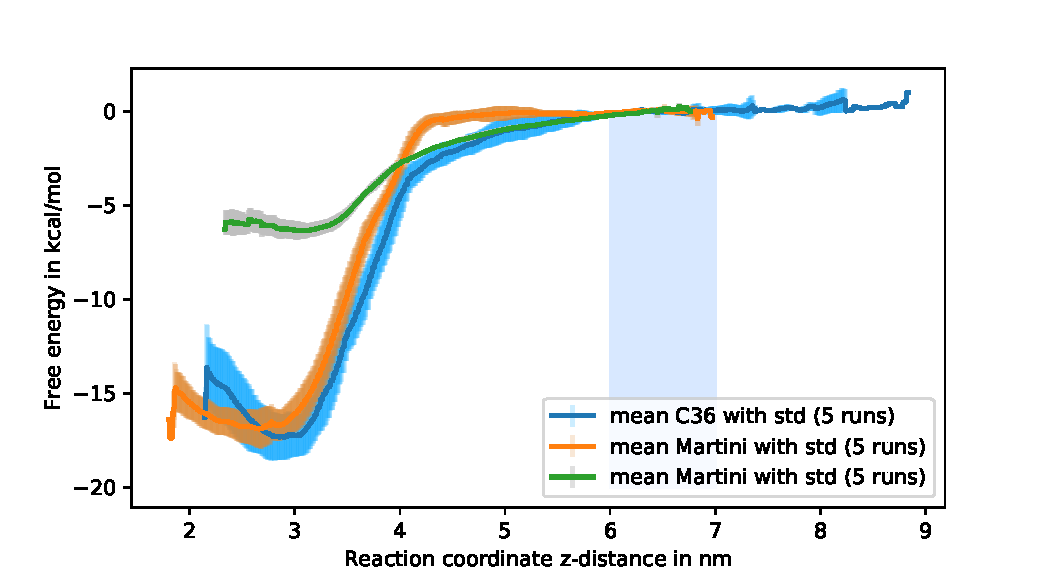
\includegraphics[width=.8\textwidth]{figures/results/umbrella}
	\captionof{figure}{Free energy profiles of basic patch in different force fields}
	\label{umbrella:profiles}
\end{figure}
%
%
%